\chapter{The PI4-Cluster Testbed}

\section{Setting Up Dual Boot}

First install Ubuntu. When asked for partitioning the disk, choose \lstinline{manual}, select the disk and confirm creating a new empty partition with \lstinline{yes}. Select the newly created empty partition followed by \lstinline{create a new partition} and set a size for it. The type should be of \lstinline{primary}, location at \lstinline{beginning} and mounting point \lstinline{root}. Finish off with \lstinline{done setting up the partition} followed by \lstinline{finish partitioning and write changes to disk}.

\begin{figure}[H]
    \centering
    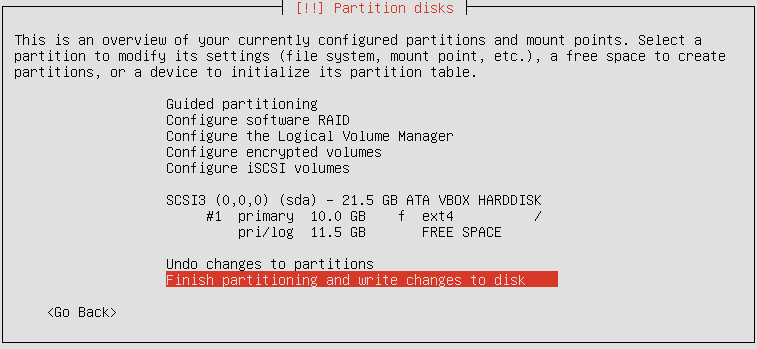
\includegraphics[width=0.75\linewidth]{ubuntu_partition}
    \captionsetup{width=0.75\linewidth}
    \caption{The partition editor for Ubuntu.}
    \label{fig:ubuntu_partition}
\end{figure}

Next, install FreeBSD. When asked for partitioning the disk, choose \lstinline{auto (UFS)} followed by \lstinline{partition}. Set a size, hit \lstinline{ok} and \lstinline{finish}.

\begin{figure}[H]
    \centering
    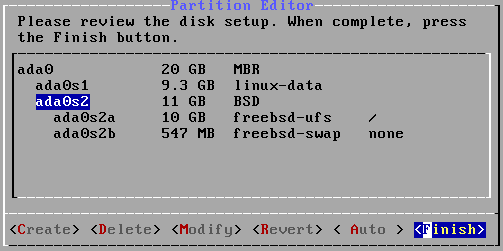
\includegraphics[width=0.75\linewidth]{freebsd_partition}
    \captionsetup{width=0.75\linewidth}
    \caption{The partition editor for FreeBSD.}
    \label{fig:freebsd_partition}
\end{figure}

After installing both systems, only Ubuntu is presented in the \gls{grub}. To add FreeBSD as an option, run \lstinline{sudo nano /etc/grub.d/40_custom} in Ubuntu, and add the following entry:

\begin{lstlisting}
menuentry "FreeBSD" {
    insmod ufs2
    set root=(hd0,2)
    kfreebsd /boot/loader
}
\end{lstlisting}

Then update \gls{grub} with \lstinline{sudo update-grub}. The FreeBSD option should now be available when rebooting. If the bootloader won't display, hold the \lstinline{RIGHT SHIFT} key upon booting.

To enable a one-time reboot into FreeBSD from Ubuntu, run the command \lstinline{grub-editenv /boot/grub/grubenv set next_entry="FreeBSD"} and reboot with \lstinline{sudo reboot}.





\section{Compiling Mainline Kernel 5.5 for Raspberry Pi 4}


\section{Patching web10g on Mainline Kernel 5.5}